\documentclass{article}
\usepackage{graphicx}
\usepackage{amsmath}
\usepackage{bm}


\begin{document}
\section{Preface}

%\begin{figure}[htpb]
%  \centering
%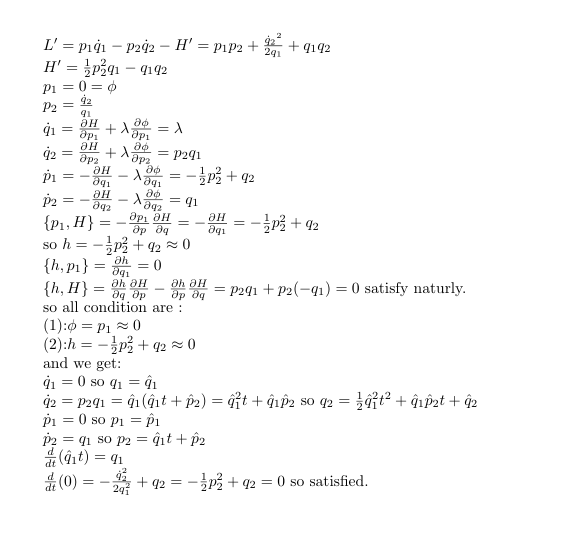
\includegraphics[width=0.5\textwidth]{Langrandian(1-1).png} 
%\caption{A Lagrangian}
%\end{figure}

From today(Nov 11) i will begin to re-learn quantum mechanics and start my note working ,try to fix the whole quantom world in my head.

\section{Wavefunction}
\subsection{Begin of the probability wave}
Discribe the probability of a particle that will appear in a place.And from the principle of quantom mechanics , consider a situation that don't procuducting any or annihilation any particle. 
\begin{align}
  \int \phi^*\phi \quad\varepsilon=1
  \label{eq:normalization}
\end{align}

That means the whole probability of a partiacle is 1 for every possimble position.
Here are some equations will be used in the next learning:

\begin{align}
\overline{(\Delta u)^2} =\overline{( u^2)}-(\bar u)^2  \\
\overline{\Delta u}=\sqrt{\overline{u^2}-{\bar u}^2}
\end{align}

These are the simplest math equations but will be used in \textbf{uncertainty relation}.

\subsection{wave function}

we call the wave function which is differ in a constant multipled are the same function:
\begin{equation}
\phi=C\phi
\end{equation}

so we call the principle is \textbf{the probability of the function waves are relatively}.

\subsection{momentum}

We all know how to define the momentum of a particle , but (consider it is the relearn note) we know the uncertainty principle,so by using \textbf{Fourier transformation}:
\begin{align}
  f(k)=\frac1{\sqrt {2\pi}}\int ^{+\infty}_{-\infty}f(x)e^{-ikx} dx \\
  f(x)=\frac1{\sqrt {2\pi}}\int ^{+\infty}_{-\infty}f(k)e^{ikx} dk 
\end{align}

and define the momentum:
\begin{equation}
  \phi(p)=\frac1{\sqrt{2\pi\hbar}}\int \phi(x)e^{\frac{-ipx}{\hbar}}dx
\end{equation}

What do $\phi(p)$ express?It express the \textbf{format of wave function in the space of momentum}.So we can calculate the momentum by:
\begin{equation}
  \overline p=\int_{p} \phi(p)^*p\phi(p)\quad\epsilon
\end{equation}

This integerallarge is defined on the space of momentum,the reason of why we not to choose to calculate the average momentum by using :$\int \phi(x)^*p\phi(x)$ is the momentum can not be certain with x at the same time.

And we also consider about the de Broglie relation:
\begin{equation}
  p=\frac{h}{\lambda} 
\end{equation}
\subsection{uncertainty relation}

The strict define of uncertainty relation:
\begin{equation}
  \Delta A\Delta B\ge\frac12|\overline{[A,B]}|
\end{equation}

The $\Delta A\Delta B$here are the $\sqrt{\overline{(\Delta A)^2}\times\overline{(\Delta B)^2}}$.

\subsection{Average of Mechanic Variable}

The define is :

\begin{equation}
\int \phi^* A \phi=\overline A
  \end{equation}
\subsection{coordinate representation}

How to express coordinate representation?It just like the relationship between physics object and coordinate base.Like how to get the part of a tensor or a part of a vector.The $\bm{\phi(t)}$ is the physics object and $\bm{\phi(x)}$ is this object in x space ,and $\bm{\phi(p)}$ is the object in momentum space. 

And the base of these projection are the base in Hilbert space.

Hilbert space:the every possimble state of wave function $\phi$.

CSCO:a set of commutating operator ,and the co-eigenstate is a base of Hlbert space. 

  \section{Shr\"odinger equation}

  \begin{equation}
    i\hbar\frac{ \partial \phi(r,t)}{ \partial t}=[-\frac{\hbar^2}{2m}\nabla+V(r,t)]\phi(r,t)
  \end{equation}

  \subsection{propagator}

  Because Shr\"odinger equation only have the 1 class derivative of time t so if we set the wave function \textbf{of free particle} at $t=0$ : $\phi(r,0)$ we can get we any time wave function $\phi(r,t)$ :
  \begin{align}
   & \phi(r,t)=\frac1{{2\pi\hbar}^{\frac32}}\int \phi(p)e^{\frac{ipr-iEt}{\hbar}}d^3p\quad E=\frac{p^2}{2m} \\
& \phi(r,0)=\frac1{{2\pi\hbar}^{\frac32}}\int \phi(p)e^{\frac{ipr}{\hbar}}d^3p \\
    \text{reverse tranformation:}&\phi(p)=\frac1{{2\pi\hbar}^{\frac32}}\int \phi(r,0)e^{\frac{-ipr}{\hbar}}d^3r \text{ put back to (13)} \\
    \phi(r,t)=& \frac1{{2\pi\hbar}^{3}}\int d^3p\int d^3r'\phi(r',0)e^{\frac{ip(r-r')-iEt}{\hbar}}
  \end{align}
  The reason of from eq(14) to eq(15) is \textbf{Fourier transformation don't rely on time t}
  and for any common situation:
  \begin{equation}
    \psi(r,t)=\frac1{{2\pi\hbar}^3}\int d^3r'\int d^3p\phi(r',t')e^{\frac{ip(r-r')-iE(t-t')}{\hbar}}
  \end{equation}

  rewrite it into form :
  \begin{align}
   \psi(r,t)=\int d^3r' G(r,r',t,t') \phi(r',t') \\
   G=\frac1{{2\pi\hbar}^3}\int e^{\frac{ip(r-r')-iE(t-t')}{\hbar}}d^3p
  \end{align}

  and the G in there is called propagator.For an eigenstate of $\hat H$ the wave function can be write as:$\psi(r,t)=\frac1{{2\pi\hbar}^{\frac32}}e^{\frac{ipr-iEt}{\hbar}}$ .

  Now look back at eq(18) we can express this equation as :Wave function of time at t is  all wave function of the particle in time t' and r' coherent superposition then spreaded to r  .

  \subsection{Time Factor}

  We set $\psi(r,t)=\psi(r)f(t)$ and consider a simple situation :V in $\hat H$ don't explicit t.And $\psi(r,t)$ is the eigenstate of E.
\begin{align}
  i\hbar\psi(r)\frac{ \partial f(t)}{ \partial t}&=[-\frac{\hbar^2}{2m}\nabla+V]\psi(r,t) \\
  E\psi(r,t)&=[-\frac{ \hbar^2}{2m}\nabla+V]\psi(r,t) \\
  f(t)&=e^{\frac{-iEt}{\hbar}}
\end{align}

so the $\psi(r,t)$ can be rewirte as :$\psi_E(r)f(t)$ For a more normalized situation,we can write any $\psi(r,t)$ into eigenstate of E:$\psi_{En}(r)$ :
\begin{align}
  \psi(r,t)&=\Sigma_n C_n\psi_{En}f_n(t)=\Sigma_n C_n\psi_{En}e^{\frac{-iE_nt}{\hbar}} \\
  |C_n|^2&=\int \psi_{En}^*\psi(r,0)
\end{align}

\subsection{Stationary state}

We call a wave function in form $\psi(r,t)=\psi(r)e^{-i\frac{Et}{\hbar}}$ as the stationary state wave function.When a particle stay in stationary state the energy of this particle is exactly can be determined.And the particle have these nature satisfied when it is a stationary particle:

(1) the probability density is not go with time:
\begin{align}
   \psi^*\psi=\rho(r) \\
\end{align}

  (2)the probability flux is not go with time :
  \begin{align}
    j_n(r,t)=\frac{i\hbar}{2m}[\psi_n\nabla\psi_n^*-\psi_n^*\nabla\psi_n]=j_n(r)
  \end{align}

  (3)any average of dynamical variables which don't dependent on time will not dependent on time:
  \begin{align}
\overline F=\int \psi(r,t)^*F\psi(r,t)=\int \psi(r)^*F\psi(r)
  \end{align}

  (4)any observed value from observable dynamical variables don't explicit t will not dependent on time.
  \section{Operator}

  \subsection{The Operator Algebra}

  Operators normally don't satisfy the law of multiple exchange.So we define the commutator:
  \begin{equation}
    [A,B]=AB-BA
  \end{equation}

  And also can de defined the linearity of operators:
  \begin{equation}
    (c_1A+c_2B)\psi=c_1A\psi+c_2B\psi
  \end{equation}

  \subsection{commutator}

Commutator is one of the important concept in QM,and there are some qualities comutator have:
\begin{align}
  [x,y(p(x))]=i\hbar\frac{ \partial y}{ \partial p(x)} \\
  [p(x),y(x)]=-i\hbar\frac{ \partial y}{ \partial x}
\end{align}

The equation(31) is the equation in coordinate representation p,and equation(32) is in the coordinate representation x.So we can find the basic law:
\begin{equation}
  [A(x),B(A(x))]=i\hbar\frac{ \partial B}{ \partial A(x)}
\end{equation}

and from the upper dicussion we know there is a strong relationship between commutator and uncertainty relation at equation(10).

And the function of a variable will commmutated with another function of the same variable
\begin{equation}
  [A(f),B(f)]=0
\end{equation}

\subsection{Some unique transform in QM}

Most of mechanics operators is hermited ,$\hat A^{\dagger}=\hat A$ for define
\begin{equation}
  \int \phi^*\hat A^{\dagger}\psi=\int (\hat A\psi)^*\psi=\int \psi^*A\psi
\end{equation}

\subsection{angular momentum in QM}

The operator of angular momentum:$\hat l=r\times\hat p=r^i\hat p^j\varepsilon_{ijk} $
Rewrite them in a sphere coordinate system,noticed that the form of $l_z$ is simple and \textbf{we know now ,the eigenstate of $l_z$ is a Spherical harmonic function $Y_{lm}$}.\textbf{NOTICE :} the eigentstate of $l_z$ can be a part of Sphereical harmonic function :$\psi=\frac1{\sqrt{2\pi}}e^{im\phi}$,and the eigenstate of $l^2$ can be another ppart of Spherical harmonic function.\textbf{So Spherical harmonic function is the co-eigenstate of both opeator :$\hat l_z,\hat l^2$}.
\begin{align}
  \hat l_zY_{lm}&=m\hbar Y_{lm} \\
  \hat l^2Y_{lm}&=l(l+1)\hbar^2Y{l,m} \\
  [\hat l^2,\hat l_i]&=0 \\
  [l_i,x^j]&=i\hbar\varepsilon_{ijk}x^{k} \\
  [\hat l_i,\hat l_j]&=i\hbar\varepsilon_{ijk}\hat l_k
\end{align}
And the define of Shperiacl harmonic function:
\begin{align}
  Y_{lm}(\theta,\phi)=(-1)^m\sqrt{\frac{(l-m)!(2l+1)}{4\pi(l+m)!}}P_l^m(cos\theta)e^{im\phi}\\
   l=0,1,2,\dots,m=-l,-l+1,\dots,l-1,l.\notag
\end{align}

And the Orthogonal normalization condition is written as:
\begin{equation}
  \int Y^*_{lm}Y_{l'm'}\;\epsilon=\delta_{ll'}\delta_{mm'}
\end{equation}

\textbf{Now I will list a important example :}

$\hat l^2 -\hat l_z^2=\hat l_x^2+\hat l_y^2$
and consider a situation($\psi=Y_{lm}$):$\int \psi^*\hat l_x^2\psi$

=$\int \phi^*\frac1{i\hbar}[\hat l_y,\hat l_z]\hat l_x\psi=\frac1{i\hbar}\int \psi^*(\hat l_y\hat l_z-\hat l_z\hat l_y)\hat l_x\psi$

=$\frac1{i\hbar}\int \phi^*\hat l_y\hat l_z\hat l_x \phi-\phi^*\hat l_z\hat l_y\hat l_x\psi$

consider $\hat l_z\hat l_x=\hat l_x\hat l_z+i\hbar\hat l_y$

=$\frac1{i\hbar}\int \psi^* \hat l_y(\hat l_x\hat l_z+i\hbar\hat l_y)\psi-\psi^*\hat l_z\hat l_y\hat l_x\psi$

=$\frac1{i\hbar}\int \psi^*\hat l_y\hat l_x\hat l_z\psi+i\hbar\psi^*\hat l_y^2\psi-\psi^*\hat l_z\hat l_y\hat l_x\psi$

=$\frac1{i\hbar}\int \psi^*\hat l_y\hat l_xm\hbar\psi+i\hbar\psi^*\hat l_y^2\psi-m\hbar\psi^*\hat l_y\hat l_x\psi$

=$\int \psi^*\hat l_y^2\psi$

so we get 
\begin{equation}
  \overline{\hat l_x^2}=\overline{\hat l_y^2}
\end{equation}

\textbf{Now consider the first equation :}

$\overline{\hat l^2}+\overline{\hat l_z^2}=2\overline{\hat l_y^2}=2\overline{\hat l_x^2}$

and $\int \psi^*\hat l^2\psi=\int \psi^*l(l+1)\hbar^2\psi=l(l+1)\hbar^2$ ; $\int \psi^*\hat l_z^2\psi=\int (\hat l_z\psi)^*\hat l_z\psi=m^2\hbar^2$

so \begin{equation}
  \overline{\hat l_x^2}=\overline{\hat l_y^2}=\frac12(l(l+1)-m^2)\hbar^2
  \end{equation}

  We know the average of angular momentum $\hat l_x$ and $\hat l_y$ is :
  $\int Y_{lm}^*\hat l_xY_{lm} \; \hat l_x=\int Y_{lm}^* \frac1{i\hbar}[\hat l_y,\hat l_z]Y_{lm}=\frac1{i\hbar}\int Y_{lm}^*\hat l_y\hat l_zY_{lm}-Y_{lm}^*\hat l_z\hat l_yY_{lm}=0$
so we get :

\begin{equation}
  \overline{\hat l_x}=\overline{\hat l_y}=0
\end{equation}

so we know the uncertainty relation between $\hat l_x$ and $\hat l_y$

\begin{align}
  \Delta{\hat l_x}\Delta{\hat l_y}=\sqrt{\overline{\hat l_x^2}-\bar {l_x}^2}\sqrt{\overline{\hat l_y^2}-\bar {l_y}^2}=\frac12(l(l+1)-m^2)\hbar
\end{align}

\subsection{Function of operator}

We can define the function of operators as :
\begin{equation}
  F(\hat A)=\Sigma_n\frac{F^n(0)}{n!}\hat A^n
\end{equation}

such as :$e^{a\frac{d}{dx}}$ is a typicaly function of operator.And the effect of this function is :
\begin{align}
  e^{a\frac{d}{dx}}\psi(x)=\Sigma_n\frac{a^n}{n!}\frac{d^n}{dx^n}\psi(x)=\psi(x+a)
  \end{align}

  so $e^{a\frac{d}{dx}}$ is the operator that move the function point from x to x+a.

  \section{symmetry of evolutioning Dynamical variables }

  \subsection{Conserved observable}

  If a average value of observable is not changed with time , thus this observable is a conserved observable.
  \begin{align}
    \frac{d}{dt}\bar A(t)=\frac1{i\hbar}\overline{[A,H]}
  \end{align}

  So if the operator of this observable is comuutated with Hamilton operator , this observable is a conserved observable.\textbf{Notice the detail of define described :AVERAGE VALUE is not go with time,not the classic type "value not go with time".The reason is the principle in QM is very different with classic mechanic.}And ofcourse a Conserved Observable can be a not certainll value,so the state of the operator observed can be the non-eigenstate of this operator.The key word is "average value".

  \subsection{Relationship Between Conserved Obserable And Energy Level Degenerate}

  There are three Theorems:

  (A)Set two non-commutated conserverd observable F and G in a system,that means:$[F,H]=0;[G,H]=0$ but $[F,G]\ne0$,thus the energy level usually degenerated.

  (B)Inference from (A):
  If a conserved observable F in a system and there is a level of energy not degenerated,then $\psi_E$ is the eigenstate of F.

  (C)virial theorem:
  \begin{equation}
    2\overline{T} =\overline{\bm{r\cdot\nabla}V}
  \end{equation}

  \subsection{* Schr\"odinger picture and Heisenberg picture}

  The average value derivative with t is $\frac{d}{dt}\overline{A(t)}=\frac1{i\hbar}\overline{[A,H]}$,now we rewrite $\psi(r,t)$ as $\hat U(t,0)\psi(r,0)$ and the $\hat U(t,0)$ here is the time shift operator and $\hat U(0,0)=1$.Now we put it back into Shr\"odinger equation:
  \begin{align}
  i\hbar\frac{ \partial} { \partial t}\psi(r,t)=\hat H\psi(r,t) \notag \\
  i\hbar\frac{ \partial }{ \partial t}\hat U(t,0)\psi(r)=\hat H\hat U(t,0)\psi(r) \notag \\
i\hbar\frac{ \partial }{ \partial t}\hat U(t,0)=\hat H\hat U(t,0) \notag 
  \end{align}

  so we get(if $\hat H$ is not go with time) :
  \begin{align}
    \hat U(t,0)=e^{\frac{-i\hat Ht}{\hbar}}
  \end{align}

  or ($\hat H$ go with time):
  \begin{align}
    \hat U(t,0)=e^{\frac{-i\int \hat Hdt}{\hbar}}
  \end{align}

  and we can proof:
  \begin{align} 
    \int\phi(r,t)^*\psi(r,t)&=\int\hat U(t,0)^*\phi(r,0)^*\hat U(t,0)\psi(r,0) \notag \\
                            &=\int \phi(r,0)^*\phi(r,0)=1
  \end{align}

  For a more common situatioin we can say the \textbf{wave function is not go woth time but operators are go with time},and we rewrite $\phi(r,t)$ into $\hat U(t,0)\psi(0)$.And the operator can be written in:
  \begin{align}
    \overline{\hat A(t)}=&\int \hat U(t,0)^*\psi(0)^*\hat A\hat U(t,0)\psi(0) \notag \\
    =&\int \psi(0)^*\hat U(t,0)^{\dagger}\hat A\hat U(t,0)\psi(0) \notag \notag \\
    =&\int \psi(0)^*\hat A(t)\psi(0) \notag
  \end{align}

   so we get the operator $\hat A(t)$ defined as 
   \begin{equation}
     \hat A(t)=\hat U(t,0)^{\dagger}\hat A\hat U(t,0)
   \end{equation}

   So the evolution equation of operators evolutino with time :
   \begin{align}
   &  \frac{d}{dt}\hat A(t)=\frac{d}{dt}(\hat U(t,0)^{\dagger}\hat A\hat U(t,0))=\frac{d \hat U(t,0)^{\dagger}}{dt}\hat A\hat U(t,0)+\hat U(t,0)^{\dagger}\hat A\frac{ d\hat U(t,0)}{dt} \notag \\
   &=\frac1{-i\hbar}\hat U(t,0)^{\dagger}\hat H\hat A\hat(t,0)+\frac1{i\hbar}\hat U(t,0)^{\dagger}\hat A\hat H\hat U(t,0)=\frac1{i\hbar}\hat U(t,0)^{\dagger}[\hat A,\hat H]\hat U(t,0) \notag
   \end{align}

   Because $\hat U(t,0)^{\dagger}\hat H\hat U(t,0)=\hat H$(easily prooved with: A and function of A are commutated) so :
   \begin{align}
     \frac{d}{dt}\hat A(t)=\frac1{i\hbar}[\hat A(t),\hat H]
   \end{align}



  Noticed that this is quite differernt from eq(49) this equation is not about average value but the eqaution of operator. And this kind of theory is called \textbf{Heisenberg Represent}.The eqaution :
  is called Heisenberg equation.As the evolution equation of operators.


  \subsection{The Relationship Between Conserved Observable and Symmetry}

  A.E.Noether:"every symmetry in nature is implicited some consverved law,the otherside every conserved law is based on one of symmetry of nature"

  (A)symmetry under transformation:
  \begin{equation}
    [\hat Q,\hat H]=0
  \end{equation}

  (B)symmetry with conserved observable:
  \begin{equation}
    [\hat F,\hat H]=0
\end{equation}

(C)symmetry of space translation:
\begin{equation}
  [p,\hat H]=0
\end{equation}

equaly with Mommentum Conserved.

(D)symmetry of space turning translation:
\begin{equation}
  [\vec l,\hat H]=0
\end{equation}

equaly to angular momentum conserved.

(E)Some other symmetry in QM:
\begin{figure}[htpb]
  \centering

\includegraphics[width=0.5\textwidth]{symmetry.png} 
\caption{picture from teacher's ppt}
\end{figure}

\subsection{*Commutation}

Here is an example.

\section{Identical Particle System and The Wavefunction}
\subsection{indentical particle and exchange operator}
An indentical particle is the particle that have all the same intrinsic properties with other particle.Two indentical particles are indistinguishiable in QM.Define an exchange operator:
\begin{equation}
  P_{ij}\psi(q_1\dots q_i\dots q_j\dots)=\psi(q_1\dots q_j\dots q_i\dots)
\end{equation}

For any observable in a system with indentical particles ,the observables have symmetry of exchange 
\begin{align}
  &P_{ij}F(q_1\dots q_i\dots q_j \dots)=F(q_1\dots q_i \dots q_j\dots) \\
  &[p_{ij},H]=0
\end{align}

For a system of indentical particles,we set if an exchange of indentical particles happend ,then the wavefunction of this system will only differed by times a constant.

\begin{align}
  &P_{ij}\psi=C\psi \\
  &P_{ij}P_{ij}\psi=C^2\psi=\psi \notag \\
  &C=\pm1
\end{align}
So that means only two posibility will happend :the wavefunction is symmetry:$\psi=P_{ij}\psi$.or the wavefunction is anti-symmetric:$-\psi=P_{ij}\psi$.

\subsection{properties of Boson and Fermion}

Boson is the particle with spin is integer times of $\hbar$.And Fermion is the particle that the spin is half-integer times of $\hbar$. But a very important nature of Boson and Fermion is Identical Boson's exchange always symmetry for a system with Boson indentical particles,and indentical Fermion's exchange in a system with indentical Fermion always anti-symmetric.

For Boson:
\begin{align}
  &\text{if $k_1\ne k_2$} \notag \\
 & \psi^S_{k_1k_2}(q_1,q_2)=\frac1{\sqrt2}(1+P_{12})\phi_{k_1}(q_1)\phi_{k_2}(q_2) \\
 &\text{if $k_1=k_2$}\notag \\
 &\psi^S_{k_1k_2}(q_1,q_2)=\phi_{k_1}(q_1)\phi_{k_2}(q_2) 
\end{align}

For Fermion:
\begin{align}
  \psi^A_{k_1k_2}(q_1,q_2)=\frac1{\sqrt2}(1-P_{12})\phi_{k_1}(q_1)\phi_{k_2}(q_2)
\end{align}

and we can see the state of Fermion at $k_1=k_2$ is not exist.\textbf{This is the Pauli principle.}

\section{Matrix}

\end{document}
